\documentclass[border=5pt]{standalone}
\usepackage{tikz}
\usetikzlibrary{arrows.meta, positioning, calc}
\usepackage{xcolor}
\usepackage{graphicx}

% Brand colors
\definecolor{Garnet}{HTML}{73000A}
\definecolor{Atlantic}{HTML}{466A9F}
\definecolor{Horseshoe}{HTML}{65780B}
\definecolor{Rose}{HTML}{CC2E40}
\definecolor{LightGray}{HTML}{ECECEC}
\definecolor{Congaree}{HTML}{1F414D}

\begin{document}
\begin{tikzpicture}[
    arr/.style={-{Stealth[length=3.5mm]}, very thick},
    lbl/.style={font=\small, fill=white, inner sep=2pt},
    imglbl/.style={font=\small\bfseries, anchor=north, inner sep=3pt},
    steplbl/.style={font=\normalsize\bfseries, rounded corners=3pt, inner sep=5pt},
    every node/.style={font=\normalsize}
]

% =============================================
% COLUMN 1: Raw Inputs
% =============================================
\node[steplbl, fill=LightGray, text=black] (inputlbl) {Inputs};

% Reference image
\node[below=0.6cm of inputlbl, anchor=north] (ref_img) {
    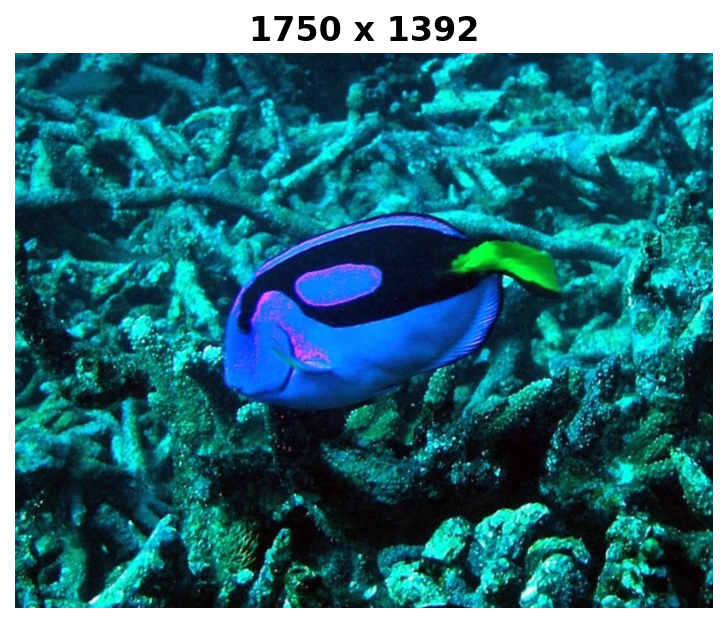
\includegraphics[width=3.8cm]{figures/dino_stage/ref_original.png}
};
\node[imglbl] at (ref_img.south) {Label Example};

% GT Mask
\node[below=0.8cm of ref_img.south, anchor=north] (gt_img) {
    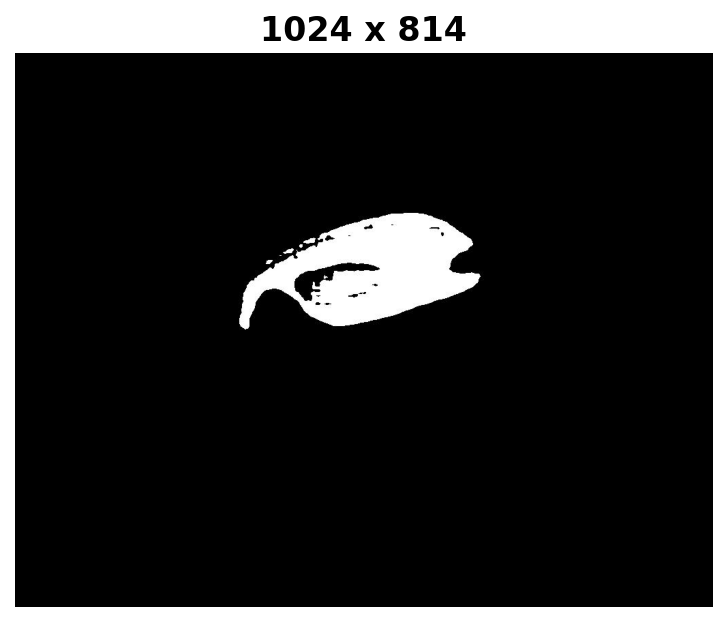
\includegraphics[width=3.8cm]{figures/dino_stage/gt_mask_original.png}
};
\node[imglbl] at (gt_img.south) {GT Mask};

% Target image
\node[below=0.8cm of gt_img.south, anchor=north] (target_img) {
    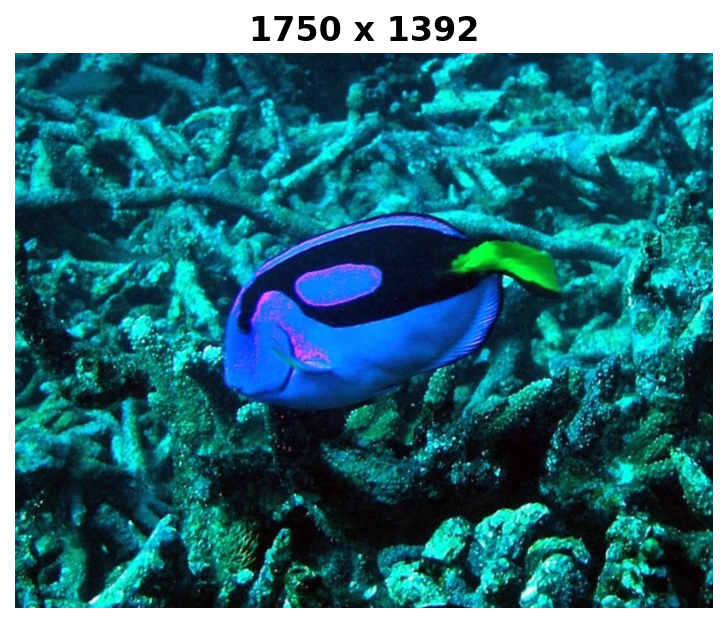
\includegraphics[width=3.8cm]{figures/dino_stage/target_original.png}
};
\node[imglbl] at (target_img.south) {Target Image};

% =============================================
% COLUMN 2: Resized 560x560
% =============================================
\node[steplbl, fill=Garnet!15, text=Garnet, right=3.5cm of inputlbl] (resizelbl) {Resize to 560$\times$560};

\node[below=0.6cm of resizelbl, anchor=north] (ref_resized) {
    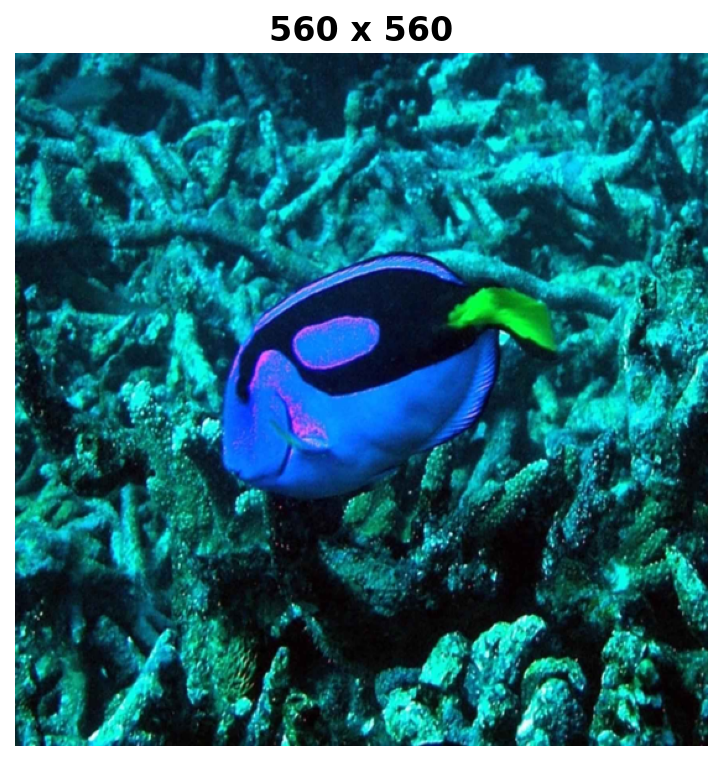
\includegraphics[width=3.8cm]{figures/dino_stage/ref_resized.png}
};
\node[imglbl] at (ref_resized.south) {Reference (560$\times$560)};

\node[below=0.8cm of ref_resized.south, anchor=north] (gt_resized) {
    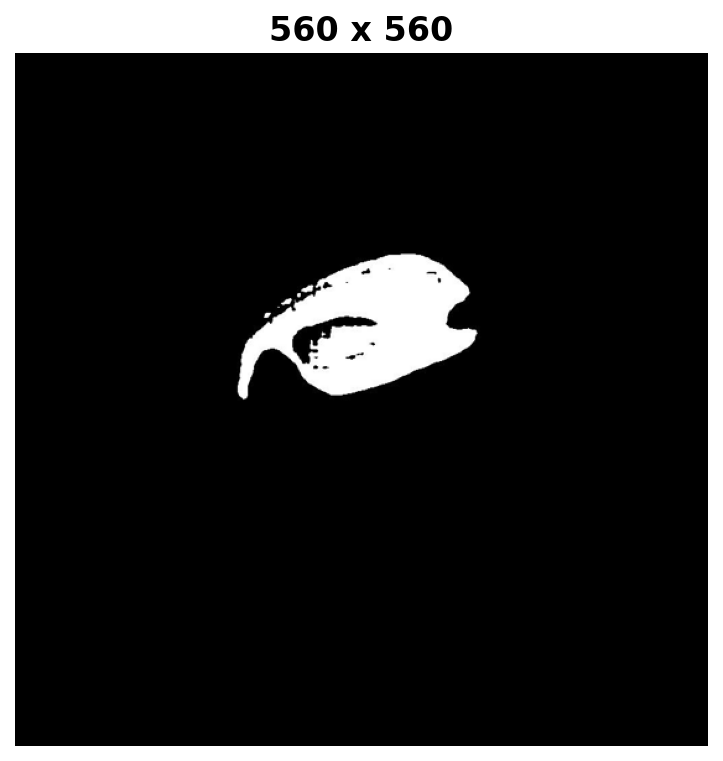
\includegraphics[width=3.8cm]{figures/dino_stage/gt_mask_resized.png}
};
\node[imglbl] at (gt_resized.south) {GT Mask (560$\times$560)};

\node[below=0.8cm of gt_resized.south, anchor=north] (target_resized) {
    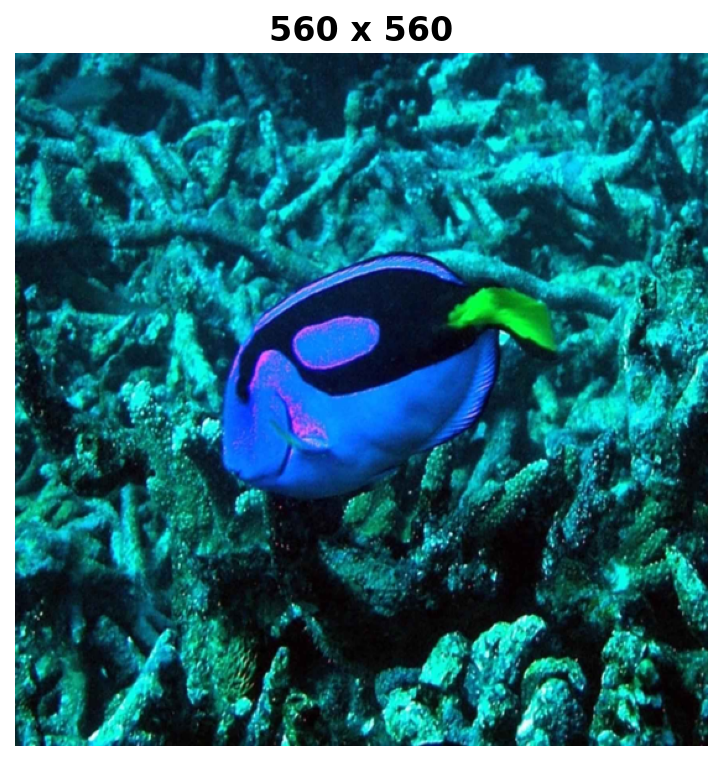
\includegraphics[width=3.8cm]{figures/dino_stage/target_resized.png}
};
\node[imglbl] at (target_resized.south) {Target (560$\times$560)};

% Arrows: raw -> resized
\draw[arr] (ref_img.east) -- (ref_resized.west);
\draw[arr] (gt_img.east) -- (gt_resized.west);
\draw[arr] (target_img.east) -- (target_resized.west);

% =============================================
% COLUMN 3: Patch Grid + GT Labels
% =============================================
\node[steplbl, fill=Atlantic!15, text=Atlantic, right=3.5cm of resizelbl] (patchlbl) {14$\times$14 Patch Grid};

\node[below=0.6cm of patchlbl, anchor=north] (ref_grid) {
    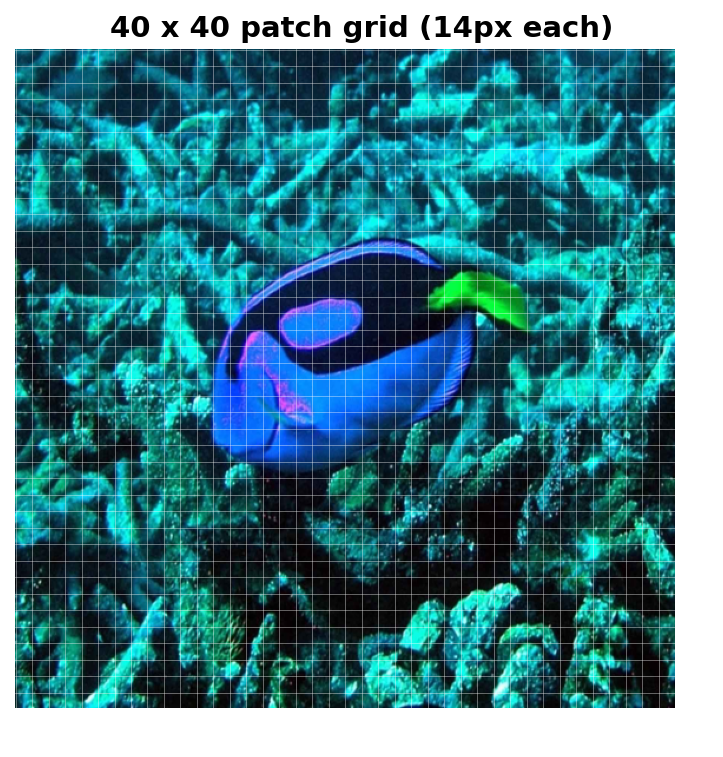
\includegraphics[width=3.8cm]{figures/dino_stage/ref_grid.png}
};
\node[imglbl] at (ref_grid.south) {40$\times$40 = 1600 patches};

\node[below=0.8cm of ref_grid.south, anchor=north] (gt_labels) {
    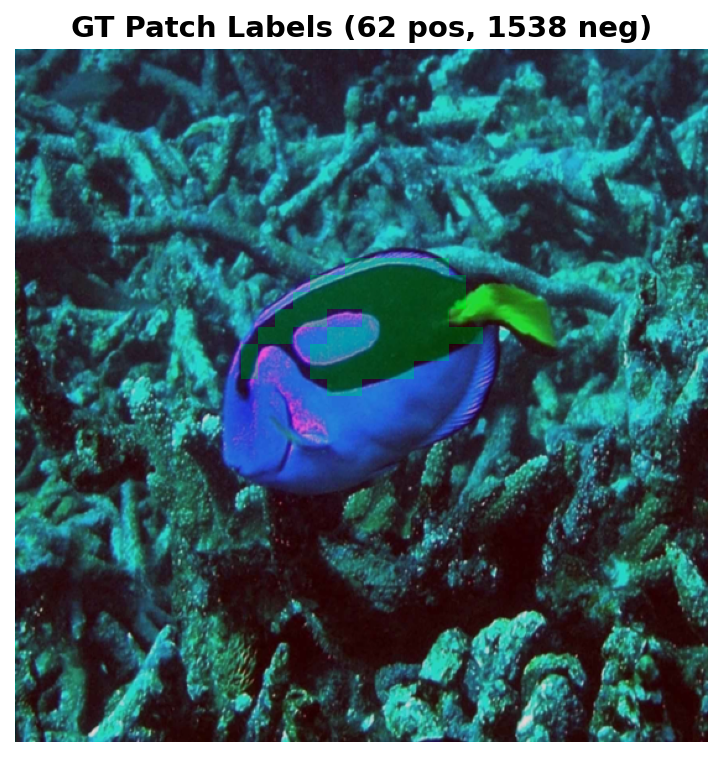
\includegraphics[width=3.8cm]{figures/dino_stage/ref_gt_patch_labels.png}
};
\node[imglbl] at (gt_labels.south) {62 pos (green), 1538 neg (red)};

\node[below=0.8cm of gt_labels.south, anchor=north] (target_grid) {
    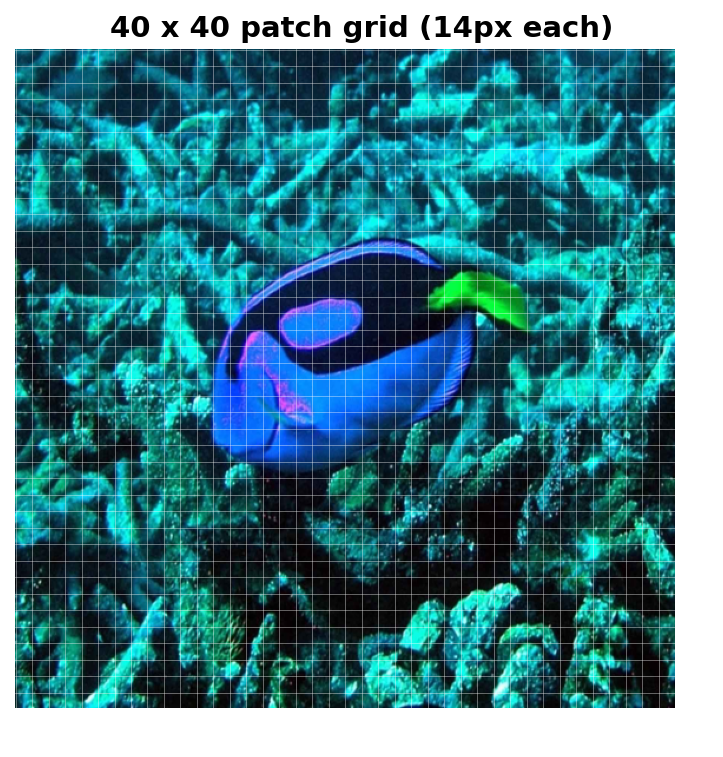
\includegraphics[width=3.8cm]{figures/dino_stage/target_grid.png}
};
\node[imglbl] at (target_grid.south) {40$\times$40 = 1600 patches};

% Arrows: resized -> grid
\draw[arr] (ref_resized.east) -- (ref_grid.west);
\draw[arr] (gt_resized.east) -- (gt_labels.west);
\draw[arr] (target_resized.east) -- (target_grid.west);

% =============================================
% COLUMN 4: DINOv2 Outputs
% =============================================
\node[steplbl, fill=Garnet!15, text=Garnet, right=3.5cm of patchlbl] (dinolbl) {DINOv2 Features};

\node[below=0.6cm of dinolbl, anchor=north] (ref_pca) {
    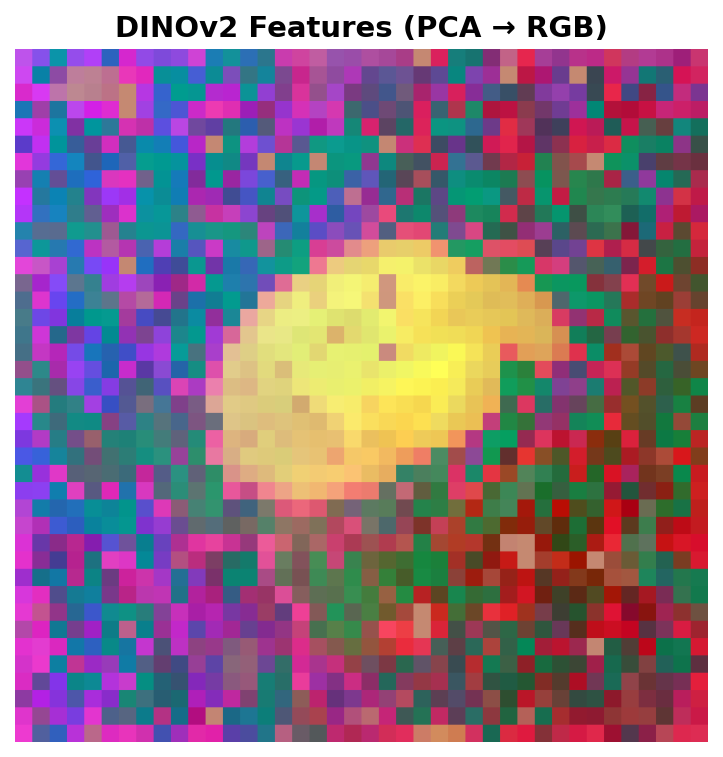
\includegraphics[width=3.8cm]{figures/dino_stage/ref_pca_features.png}
};
\node[imglbl] at (ref_pca.south) {Ref.\ features (PCA$\to$RGB)};

\node[below=0.8cm of ref_pca.south, anchor=north] (ref_overlay) {
    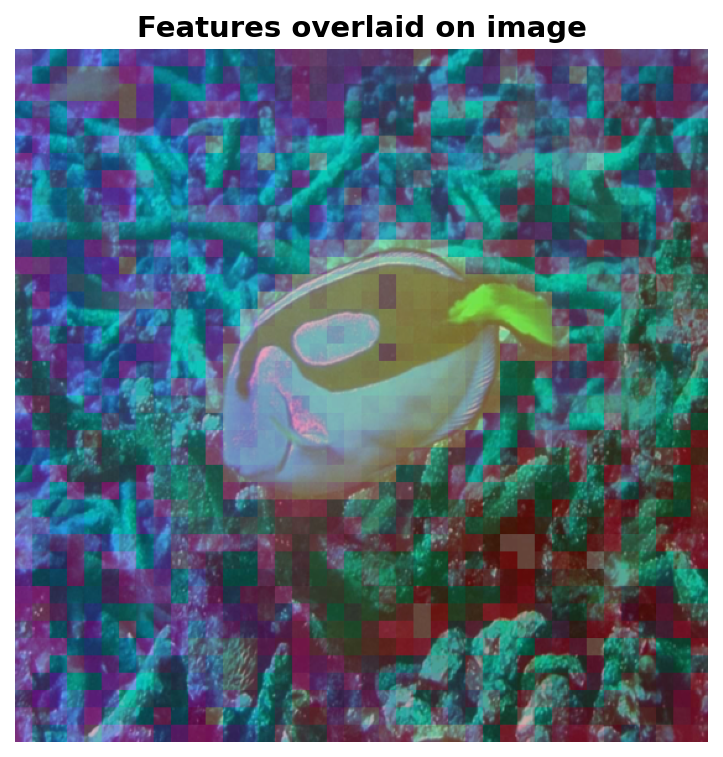
\includegraphics[width=3.8cm]{figures/dino_stage/ref_pca_features_overlay.png}
};
\node[imglbl] at (ref_overlay.south) {Features overlaid on image};

\node[below=0.8cm of ref_overlay.south, anchor=north] (target_pca) {
    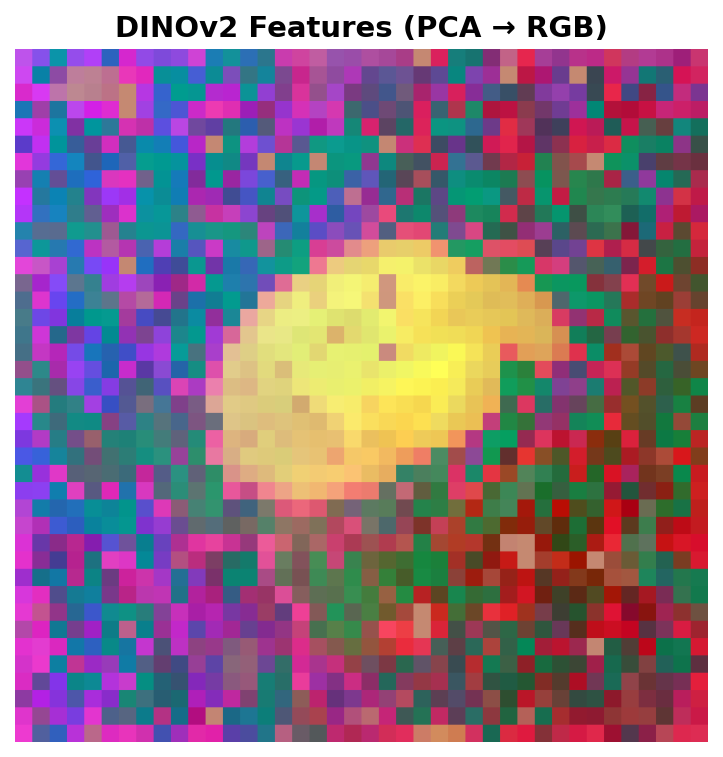
\includegraphics[width=3.8cm]{figures/dino_stage/target_pca_features.png}
};
\node[imglbl] at (target_pca.south) {Target features (PCA$\to$RGB)};

% Arrows: grid -> DINOv2
\draw[arr] (ref_grid.east) -- (ref_pca.west);
\draw[arr, dashed, Atlantic] (gt_labels.east) -- (ref_overlay.west)
    node[lbl, midway, above=0.1cm, text=Atlantic] {labels patches};
\draw[arr] (target_grid.east) -- (target_pca.west);

% =============================================
% Output annotation
% =============================================
\node[font=\small, text=Garnet, anchor=north, text width=4cm, align=center]
    at ([yshift=-0.3cm]target_pca.south) {Each image $\to$ 1600 $\times$ 1536\\feature matrix};

\end{tikzpicture}
\end{document}
